\chapter{Environment, Safety, and Health}
\label{vl:tc-ESH}


A strong \dword{esh} program is essential to successfully complete
\dword{lbnf} and \dword{dune} at \surf, which are hosted by
\fnal.  \dword{lbnf}/\dword{dune} is internationally designed,
coordinated and funded through collaborating laboratories and
universities.  \dword{lbnf} comprises the
world's highest intensity neutrino beam at \fnal and the
infrastructure necessary to support the experimental detectors at
\surf. The \dword{dune} project is committed to ensuring a
safe work environment for \dword{dune} workers at all
institutions and to protecting the public from hazards associated with
constructing and operating \dword{dune}.  Accidents and
injuries are preventable, and we must work together to
establish a workplace free of injuries.  Finally, all work must be
performed so the quality of the environment is preserved
and property damage prevented.

\fnal and \dword{dune} are committed to protecting the health and
safety of staff, the community and the environment, as stated in the
\dword{lbnf}/\dword{dune} integrated \dword{esh} plan.  The
\dword{esh} program complies with applicable standards and local,
state and federal legal requirements through the \fnal work smart set
of standards and the contract between Fermi Research Alliance and the
\dword{doe} Office of Science (FRA-DOE). \fnal, as the host
laboratory, established the South Dakota Services Division to provide
facility support.  The South Dakota Services Division is responsible
for \dword{lbnf}/\dword{dune} operations at \surf.

The \fnal \dword{esh} program strives to prevent injuries or illness and seeks to
continually improve safety and health management.  To the maximum
practical extent, all hazards must be eliminated or minimized through
substitution, engineering or administrative controls.  Where
engineering or administrative controls are not feasible, \dword{ppe}
must be used.

The \dword{esh} management system is designed to work hand in hand
with the \surf emergency management systems to protect the public,
workers and environment; ensure compliance with the FRA-DOE contract
and \fnal Work Smart standards; and improve \fnal's and \dword{dune}'s
ability to meet or exceed customer expectations. Doing so helps in
executing the scientific mission.  \fnal uses a set of criteria to
plan, direct, control, coordinate, assure and improve how \dword{esh}
policies, objectives, processes and procedures are established,
implemented, monitored and achieved.

The \fnal facilities at \surf are, moreover, subject to the requirements of the
\dword{doe} Workers Safety and Health Program, Title 10, Code Federal
Regulations, Part 851 (10 CFR 851). These requirements are
promulgated through the \fnal Director's Policy Manual\footnote{\fnal
  Director's Policy Manual is:
  http://www.fnal.gov/directorate/Policy\_Manual.html}, and the \fnal
\dword{esh} Manual\footnote{\fnal ES\&H Manual is:
  http://esh.fnal.gov/xms/ESHQ-Manuals/feshm} (\dword{feshm}), which align with
the \surf \dword{esh} Manual.


\section{\dword{dune} \dword{esh} Management and Oversight}

The \dword{tcoord} and \dword{ipd} have responsibility for
implementation of the \dword{dune} \dword{esh} program.  The
\dword{lbnf}/\dword{dune} \dword{esh} Manager reports directly to the
\dword{tcoord} and \dword{ipd} and is responsible for providing
\dword{esh} support and oversight for development and implementation
\dword{dune} \dword{esh} program. The \dword{dune} \dword{esh}
Coordinators report to the \dword{lbnf}/\dword{dune} \dword{esh}
Manager and have primary responsibility for \dword{esh} support and
oversight of the \dword{dune} \dword{esh} program for all activities
at collaborating institutions and at \dword{lbnf}/\dword{dune}
facilities located at \surf.

Additional \dword{esh} Subject Matter Experts (SME) are available to provide
supplemental support to the project through the \fnal \dword{esh}
Section. The \fnal \dword{esh} Section, DOE-Fermilab Site Office, CERN and
\surf will provide supplemental \dword{esh} oversight to validate
implementation of the \dword{dune} \dword{esh}  program.

The \dword{dune} \dword{esh} Plan 
defines the \dword{esh} requirements applicable to 
installation activities at the \surf site. Regular \dword{esh} walkthroughs
will be conducted by \dword{dune} \dword{esh} management personnel. All
findings will be documented utilizing the \fnal Predictive
Solutions database system.

Figure~\ref{fig:dune_esh} shows the \dword{dune} \dword{esh} organization.
\begin{dunefigure}[\dword{dune} \dword{esh}]{fig:dune_esh}
  {The high level \dword{dune} \dword{esh} organization.}
  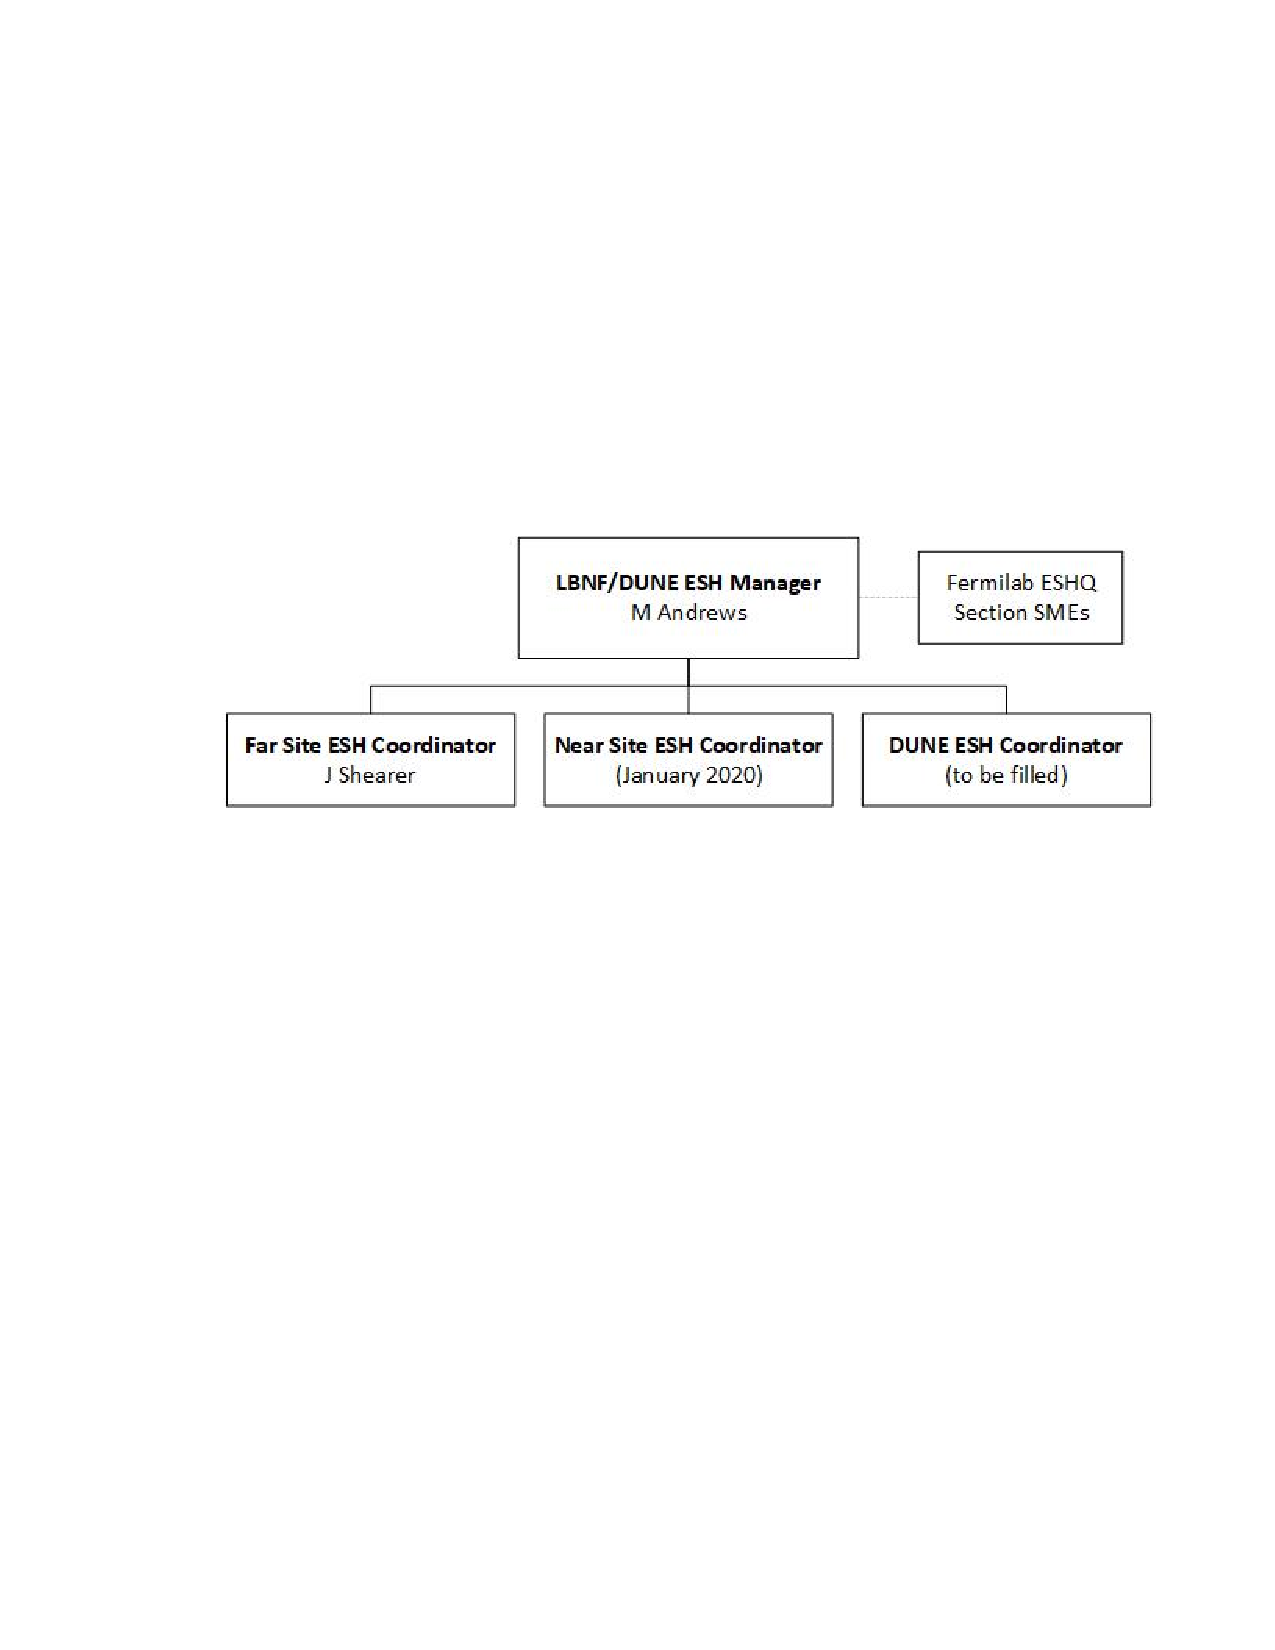
\includegraphics[width=0.85\textwidth]{dune_esh_org.pdf}
\end{dunefigure}




\section{Hazard Analysis Report}

A key element of an effective \dword{esh} program is the hazard
identification process. Hazard identification allows production of a
list of hazards within a facility, so these hazards can be screened
and managed through a suitable set of controls.

The \dword{lbnf}/\dword{dune} project completed a hazard analysis
report to ensure that identified hazards are mitigated early in the
the design process.  The focus of the report is on process hazards,
not activity hazards that are typically covered in a job hazard
analysis.  The hazard analysis report has been completed, identifying
hazards anticipated in the project's construction and operational
phases.

The hazard analysis report then looks at the consequences of a hazard
to establish a pre-mitigation risk category. Proposed mitigation is
applied to hazards of concern to reduce risk. and then establishes A
post-mitigation risk category is then established.

As the \dword{dune} design matures, the hazard analysis report will be updated to ensure
that all hazards are properly identified and controlled through
design and safety management system programs.  In addition, some
sections of the hazard analysis report are used to meet the safety requirements as
defined in 10 CFR 851 and \dword{doe} Order 420.2C, Safety of
Accelerator Facilities.  Table~\ref{tab:hazards} summarizes these
hazards.  The sections following the table describe in more detail the hazards that
are most applicable to \dword{dune} activities and the
design and operational controls used to mitigate these hazards. The
results of these evaluations confirm that the potential risks from
construction, operations, and maintenance are acceptable.
\begin{dunetable}
  [Hazard List] {|p{0.42\textwidth}|p{0.35\textwidth}|p{0.35\textwidth}|}
  {tab:hazards} {List of identified hazards}
  HA-1 (Construction) & HA-2 (Natural Phenomena) & HA-3 (Environmental)   \\ \toprowrule
  Site Clearing, Excavation, Mining, Tunneling (explosives), Vertical/Horizontal Conveyance Systems,
  Confined space, Heavy Equipment, Work at Elevations (steel, roofing), Material Handling (rigging)
  Utility interfaces, (electrical, steam, chilled water), Slips/trips/falls, Weather related conditions
  Scaffolding, Transition to Operations, Radiation Generating Devices &
  Seismic, Flooding, Wind, Lightning, Tornado &
  Construction impacts,
  Storm water discharge (construction and operations), Operations impacts, Soil and groundwater activation/contamination,
  Tritium contamination, Air activation, Cooling water activation (HVAC and Machine),
  Oils/chemical leaks or spills, Discharge/emission points (atmospheric/ground)\\ \colhline
  HA-4 (Waste) & HA-5 (Fire) & HA-6 (Electrical)   \\ \toprowrule
  Construction Phase, Facility maintenance, Experimental Operations, Industrial, Hazardous, Radiological &
  Facility Occupancy Classification, Construction Materials, Storage, Flammable/combustible liquids,
  Flammable gasses, Egress/access, Electrical, Lightning, Welding/cutting/brazing work, Smoking  &
  Facility, Experimental, Job built Equipment, Low Voltage/High Current, High Voltage/High Power,
  Maintenance, Arc flash, Electrical shock, Cable tray overloading/mixed utilities, Exposed 110V,
  Stored energy (capacitors \& inductors), Be in contactors   \\ \colhline
  HA-7 (Mechanical) & HA-8 (Cryo/ODH) & HA-9 (Confined Space)   \\ \toprowrule
  Construction Tools, Machine Shop Tools, Industrial Vehicles, Drilling, Cutting, Grinding,
  Pressure/Vacuum Vessels and Lines, High Temp Equipment (Bakeouts) &
  Thermal, Cryogenic systems, Pressure, Handling and Storage,
  Liquid argon/nitrogen spill/leak, Use of inert gases (argon, nitrogen, helium), Specialty gases &
  Sumps, Utility Chases        \\ \colhline
  HA-11 (Chemical) & HA-14 (Laser) & HA-15 (Material Handling)   \\ \toprowrule
  Toxic, Compressed gas, Combustibles, Explosives, Flammable gases, Lead (shielding), Cryogenic &
  Alignment Laser, Testing and Calibration, Magnetic Fields, Calibration \& Testing &
  Overhead cranes/hoists, Fork trucks, Manual material handling, Delivery area distribution,
  Manual movement of materials, Hoisting \& Rigging, Lead, Beryllium Windows,Oils, Solvents, Acids,
  Cryogens, Compressed Gases   \\ \colhline
  HA-16 (Experimental Ops) &  &    \\ \toprowrule
  Electrical equipment, Water Hazard, Working from heights (scaffolding/lifts), Transportation of hazardous materials,
  Liquid Argon/Nitrogen, Chemicals (Corrosive, Reactive, Flammable), Elevations, Ionizing radiation,
  Ozone production, Slips, trips, falls, Machine tools/hand tools, Stray static magnetic fields, Research gasses (Inert, Flammable) &
  &   \\ \colhline
\end{dunetable}

\subsection{Construction Hazards (\dword{lbnf}/\dword{dune} HA-1)}

The project will use the existing work planning and
control process for the laboratories along with a construction project safety and health
plan to communicate these policies and procedures as required by \dword{doe}
Order 413.3b. The installation and construction hazards
anticipated for the \dword{lbnf}/\dword{dune} project include the following:
\begin{itemize}
 \item Site clearing,
 \item Excavation,
 \item Installing vertical/horizontal conveyance systems,
 \item Confined space,
 \item Heavy equipment operation,
 \item Work at elevation (erecting steel, roofing),
 \item Material handling (rigging),
 \item Utility interfaces (electrical, chilled water, ICW, natural gas),
 \item Slips/trips/falls,
 \item Weather related conditions,
 \item Scaffolding,
 \item Transition to operations,
 \item Devices generating radiation.
\end{itemize}

To reduce risks from construction hazards, \fnal will use
engineered and approved excavation and fall protection systems.  Heavy
equipment will use required safety controls. \fnal's
construction safety oversight program includes periodic evaluation of
the construction site and construction activities, hazard analysis for
all subcontractor activities, and frequent \dword{esh} communications at the
daily tool box meetings of subcontractors.

\subsection{Natural Phenomena (\dword{lbnf}/\dword{dune} HA-2)}

The \dword{lbnf}/\dword{dune} design will be governed by the International Building
Code, 2015 edition; \dword{doe} Standard (STD)-1020, 2016 edition,
Natural Phenomena Hazard Analysis and Design Criteria for \dword{doe}
Facilities, guided the design in meeting the
natural phenomena hazard requirements.  The International Building Code specifies design
criteria for wind loading, snow loading, and seismic events.

\dword{lbnf}/\dword{dune} was determined to be a low hazard,
performance category 1 facility according to the \dword{doe}
STD-1021-93. \dword{lbnf}/\dword{dune} areas will contain small
quantities of activated, radioactive, and hazardous chemical
materials. Should a natural phenomenon hazard cause significant
damage, the impact will be mission related and will not pose a hazard
to the public or the environment.

\subsection{Environmental Hazards (\dword{lbnf}/\dword{dune} HA-3)}

Environmental hazards from \dword{dune} include potentially releasing
chemicals to soil, groundwater, surface water, air, or sanitary sewer
systems that could, if not controlled, exceed regulatory limits.

\fnal maintains an environmental management system equivalent to
ISO 14001, consisting of programs for protecting the environment,
assuring compliance with applicable environmental regulations and
standards, and avoiding adverse environmental impact through continual improvement.  These programs are documented in the 8000
and 11000 series of chapters in the \dword{feshm}.  The environmental
mitigation plan also meets federal and state regulations.


\subsection{Waste Hazards (\dword{lbnf}/\dword{dune} HA-4)}

Waste related hazards from \dword{dune} include the potential for releasing
waste materials (oils, solvents, chemicals, and radioactive material)
to the environment, injury to personnel, and reactive or
explosive event. Typical initiators will be transportation accidents,
incompatible materials, insufficient packaging/labeling, failure of
packaging, and a natural phenomenon.

During installation and \dword{dune} operation, we anticipate 
few hazardous materials will be used. Such materials
include paints, epoxies, solvents, oils, and lead in the form of
shielding. No current or anticipated activities at \dword{dune} 
would expose workers to levels of contaminants (dust, mists, or fumes)
above regulatory limits.

The \dword{esh}\&Q section industrial hygiene group and hazard control
technology team manage the program and guide 
collaborators subject to
waste-related hazards.  Their staff identify workplace
hazards, help identify controls, and monitor
implementation. Industrial hygiene hazards will be evaluated,
identified, and mitigated as part of the work planning and control
hazard assessment process.

\subsection{Fire Hazards (\dword{lbnf}/\dword{dune} HA-5)}

The probability of a fire at \dword{lbnf}/\dword{dune} is very low,
similar to that of present neutrino detector operations for MINOS,
NOvA, and MicroBooNE at \fnal.


Fire hazards have been evaluated and addressed to comply with \dword{doe}
Order 420.1C, Facility Safety, Chapter II and \dword{doe}-STD 1066, Fire
Protection Design Criteria.  The intent of these documents is to meet
\dword{doe}'s highly protected risk (HPR) approach to fire protection.  In
addition, the National Fire Protection Association Standard
520, Standard on Subterranean Spaces, was used in developing the
basis for design related to fire protection/life safety.

The combustible loads and the use of flammable and/or reactive
materials in the \dword{lbnf}/\dword{dune} facility are controlled following
the International Building Code building occupancy
classification. Certain ancillary buildings outside the main structure
may be classified as higher hazard areas (Use Group H occupancy),
including the gas cylinder and chemical storage rooms, because they
hold more concentrated quantities of flammable or combustible
materials.  The control area concept used in the International Building Code and National Fire Protection Association standards will be followed for hazardous chemical use and storage
areas to provide the most flexibility and control of
materials by allowing inventory thresholds per control area.  The
\dword{lbnf}/\dword{dune} facility will be equipped with fire detection systems and
alarm systems that will monitor water flow in case of fire suppression
activation as well as monitor control valves and detection systems.

Audible/visual alarm notification devices will alert building
occupants.  Manual pull stations for the fire alarms will be installed
at all building exits.  Following National Fire Protection Association 90A, air handling
systems will have photoelectric smoke detectors.  Smoke detection
will be provided in areas with highly sensitive electronic
equipment.  Combinations of audible/visual alarm notification devices will
be set up throughout the underground enclosures and service buildings
to alert occupants. All fire alarm signals will report through a
centralized system at \surf.  Fire alarm and supervisory signals will
be transmitted to internal and external emergency responders using
the campus reporting system.

While fixed fire protection systems afford an excellent level
of protection, additional strategies include operational controls
that minimize combustible materials, adequately
fused power supplies, fire safety inspections, and operational
readiness reviews will be used to further reduce fire hazards
within the facility following \dword{doe} highly protected risk methods.

Experimental cabling will meet the requirements of the National Fire Protection Association 70 and National
Electrical Code, 2015 edition.  Preferred cables should be fire
resistant, using appropriately designated cable types for plenum
or general-purpose cables.  When there is a
large investment in equipment for
experiment power or computer rack systems or when equipment is
custom made (as opposed to off-the-shelf commercial electronics), a
device to detect faults or smoke in the system should be provided.
This device should also shut down the individual rack or racks when 
smoke or faults are detected.


\subsection{Electrical Hazards (\dword{lbnf}/\dword{dune} HA-6)}

\dword{lbnf}/\dword{dune} will have significant facility-related systems and
subsystems that produce or use high voltage, high current, or high
levels of stored energy, all of which can present electrical hazards
to personnel. Electrical hazards include electric shock and arc flash
from exposed conductors, defective and substandard equipment, lack of
training, or improper procedures.

\fnal has a well-established electrical safety program that
incorporates deenergizing equipment, isolation barriers, personal
protective equipment, and training. The cornerstone of the program is
the lockout/tagout following the \dword{feshm}
Chapter 2100, \fnal Energy Control Program (Lockout/Tagout).

Design, installation, and operation of electrical equipment will comply with the National Electrical code (NFPA 70), applicable
parts of Title 29 Code of Federal Regulations, Parts 1910 and 1926,
National Fire Protection Association 70E, and \fnal electrical safety policies documented in the
\dword{feshm} 9000 series chapters. Equipment procured from outside vendors or
international in-kind partners will be either certified by a
nationally recognized testing laboratory, conform to
international standards previously evaluated and deemed equivalent to
US standards, or inspected and accepted using \fnal's
electrical equipment inspection policies outlined in \dword{feshm} 9110,
Electrical Utilization Equipment Safety.


\subsection{Noise/Vibration/Thermal/Mechanical (\dword{lbnf}/\dword{dune} HA-7)}

Hazards include overexposure of personnel noise and vibrations as
specified by the American Conference of Governmental Industrial
Hygienists and US Occupational Safety and Health Administration
(OSHA), which set noise limits to avoid permanent hearing loss, also
known as permanent threshold shift . Vibration of equipment can
contribute to noise levels and could damage or interfere with
sensitive equipment.

\dword{lbnf}/\dword{dune} will use a wide variety of equipment that will
produce a wide range of noise and vibration. Support equipment, such
as pumps, motors, fans, machine shops, and general HVAC, all contribute
to point source and overall ambient noise levels. While noise will
typically be below the ACGIH and OSHA 8-hour time weighted average,
certain areas with mechanical equipment could exceed that criterion
and will require periodic monitoring, posting, and use of
protective equipment. Ambient background noise is more a concern for collaborator comfort, stress levels, and fatigue.

The detector facilities use a wide variety of noisy equipment. Pumps,
fans, and machine shop devices, among others, are possible sources of
noise levels that might exceed the \fnal noise action levels. \dword{feshm}
Chapter 4140, Hearing Conservation, details requirements for reducing
noise and protecting personnel exposed to excessive noise
levels. Warning signs are posted wherever hazardous noise levels may
occur, and hearing protection devices are readily
available. Ways to reduce noise and vibration will be
incorporated into the \dword{lbnf}/\dword{dune} design. These techniques include using
low noise/vibration producing equipment, especially for fans in the
HVAC equipment, isolating noise producing equipment by segregating
or enclosing it, and using sound deadening materials on walls and
ceilings.

\subsection{Cryogenic/Oxygen Deficiency Hazard (\dword{lbnf}/\dword{dune} HA-8)}

The \dword{lbnf}/\dword{dune} project will use large volumes of liquid
argon, nitrogen, and helium within the Far Site facilities. Cryogenic
hazards could include oxygen deficient atmospheres due to

failure of
the cryogenic systems, thermal (cold burn) hazards from cryogenic
components, and pressure hazards. Initiators could include the failure
or rupture of cryogenic systems from overpressure, failure of
insulating vacuum jackets, mechanical damage or failure, deficient
maintenance, or improper procedures.

Cryogenic liquids and gasses are extremely dangerous to humans,
destroying tissue, and can damage materials and equipment past repair
by altering characteristics and properties (like size, strength, and
flexibility) of metals and other materials.

Although cryogens are used extensively at \fnal, quantities that may be used within a facility are strictly limited. Uses
beyond defined limits require oxygen deficiency hazard 
analyses and using ventilation, oxygen deficiency monitoring, or
other controls.

Cryogenic systems are subject to formal project review, which includes
independent reviews by a subpanel of the Cryogenic Safety Subcommittee
following National Fire Protection Association Chapter 5032, Cryogenic
System Review. The members of this panel have relevant knowledge in
appropriate areas. They review the system safety documentation,
\dword{odh} analysis documentation, and the equipment before new
systems are permitted to begin the cool down process.

\fnal has developed and successfully deployed \dword{odh} monitoring
systems throughout the laboratory to support its current cryogenic
operations. The systems provide both local and remote alarms when
atmospheres contain less than 19.5\% oxygen by volume.

\fnal has a mature training program to address cryogenic safety
hazards. Key program elements include \dword{odh} training,
pressurized gas safety, and general cryogenic safety.


\subsection{Confined Space Hazards (\dword{lbnf}/\dword{dune} HA-9)}

Hazards from confined spaces could result in death or injury from
asphyxiation, compressive asphyxiation, smoke inhalation, or impact
with mechanical systems. Initiators would include failure of cryogenic
systems that are releasing liquid, gas, fire, or failure of mechanical
systems.

The \fnal confined space program is outlined in \fnal Environmental
and Safety Manual Chapter 4230, Confined
Spaces. \dword{lbnf}/\dword{dune} facilities will be incorporated into
this program. The emphasis at the \dword{lbnf}/\dword{dune} design
phase will be to create the minimum number of confined spaces by
clearly articulating the definition of confined spaces to facility
designers to assure that such spaces have adequate egress, mechanical
spaces are adequately sized, and, wherever possible, no confined space
created at all. During facility operations, the existing campus
confined space program, along with appropriate labeling of confined
spaces, work planning and control, and entry permits will be used to
control access to these spaces.


\subsection{Chemical/Hazardous Materials Hazards (\dword{lbnf}/\dword{dune} HA-11)}

The \dword{dune} facility anticipates minimal use of chemical and hazardous
materials. Materials like paints, epoxies, solvents, oils, and lead
shielding may be used during construction and operation of the
facility. Exposure to these materials could result in injury; 
exposure could also exceed regulatory limits. Initiators could be
experimental operations, transfer of material, failure of packaging,
improper marking/labeling, reactive or explosive event, improper
selection of or lack of personal protective equipment, or a
natural phenomenon.

\fnal maintains an database of hazardous chemicals in compliance
with the requirements imposed by 10 CFR 851 and \dword{doe} orders. In
addition to an inventory of chemicals at the facility, copies of each manufacturer's safety data sheets are
maintained. Reviews of conventional safety measures at the
facilities show that using these chemicals does not warrant special
controls other than appropriate signs, procedures, appropriate use of
personal protective equipment, and hazard communication training. \dword{dune}
will also supply safety data sheet documentation to the \surf \dword{esh} department for all
chemicals and hazardous materials that arrive on site.

The industrial hygiene program, detailed in the \dword{feshm} 4000 series
chapters, addresses potential hazards to workers using such
materials. The program identifies how to evaluate workplace hazards
when planning work and the controls necessary to either eliminate or mitigate
these hazards to an acceptable level.

Specific procedures are also in place for safe handling, storing,
transporting, inspecting, and disposing of hazardous materials. These
are contained in the \dword{feshm} 8000 and 10000 series chapters,
Environmental Protection and Material Handling and Transportation,
which describe how to comply with the standards set by the Code of
Federal Regulations, Occupational Safety and Health Standards, Hazard
Communication, Title 29 CFR, Part 1910.1200.


\subsection{Lasers \& Other Non-Ionizing Radiation Hazards (\dword{lbnf}/\dword{dune} HA-14)}

Production and delivery of Class 3B and Class 4, near-infrared, UV,
and visible lasers must be completely contained in
transport pipes or designated enclosures for the Class 3b and Class 4
lasers, thus creating a laser controlled area. (This will be in
accordance with \fnal \dword{feshm} chapter 4260.)  Establishing the laser controlled area
prevents areas around it from exceeding the maximum
permissible exposure as set by the \fnal laser safety officer.

\subsection{Material Handling Hazards (\dword{lbnf}/\dword{dune} HA-15)}

\dword{dune} will require a significant amount of manual and mechanical
material handling during the construction, installation, and operations
phases.  The consequences of these hazards include serious injury or
death to equipment operators and bystanders, damage to equipment and
structures, and interruption of the program.  Additional material
handling hazards from forklift and tow cart operations include injury
to the operator or personnel in the area and contact with equipment or
structures. Cranes and hoists will be used during fabrication,
testing, removal, and installation of equipment. The error precursors
associated with this type of work may include irregular shaped loads,
awkward load attachments, limited space, obscured sight lines, and
poor communication.  The material or equipment being moved is
typically one of a kind, expensive or of considerable programmatic
value, and without dedicated lifting points or an obvious center
of gravity.

Lessons learned from across the \dword{doe} complex and OSHA have been
evaluated and incorporated into the \fnal material handling
programs documented in the \dword{feshm} 10000 series chapters.  The
laboratory limits personnel with access to mechanical material
handling equipment like cranes and forklifts to those who have
successfully completed the laboratory's training programs and
demonstrated competence in operating this equipment.


\subsection{Experimental Operations (\dword{lbnf}/\dword{dune} HA-16)}

Experimental activity undertaken at \dword{lbnf}/\dword{dune} will be fully reviewed
under the operational readiness clearance (ORC) process and by other
experts as needed (e.g., representatives from
electrical safety, fire safety, environmental compliance, industrial
hygiene, cryogenic safety, and industrial safety), to identify and
manage the hazards of each experimental operation. The shift leader
will ensure that all safety reviews take place for each
activity and that any issues are appropriately addressed. The ORC
process will document these reviews, covering the necessary controls
and management approval to proceed.

Typically, the ORC process evaluates the scope of the proposed
experimental activity and identifies the hazards and controls to
mitigate them. The process ensures that collaborators are properly trained, that
qualified, hazardous material is kept to a minimum, that engineering
controls are deployed as a preferred mitigation, and that personnel
protective equipment is appropriate for the hazard.

\section{National Environmental Protection Act Compliance}

In compliance with the National Environmental Protection Act 
and in accordance with \dword{doe} Policy 451.1, the
\dword{lbnf}/\dword{dune} project performed an evaluation of potential
environmental impacts during construction and operation of the
project.  An environmental assessment has been prepared on the potential environmental impacts and the safety and health
hazards identified during the design, construction, and operating
phases of \dword{lbnf}/\dword{dune}.  The environmental assessment presented an analysis of the potential
environmental consequences of the facility and compared them to the
consequences of a No Action Alternative. The assessment included
detailed analysis of all potential environmental, safety, and health
hazards associated with construction and operation of the facility.
The environmental assessment has been completed and a finding of no significant impact (FONSI)
issued in September 2015.

\section{Codes/Standards Equivalencies}
\label{sec:esh_codes}

\dword{dune} will rely on significant contributions from international
partners. In many cases, an international partner will contribute
equipment for installation at \fnal built following one of the
international standards or directives. \fnal has established a
process, detailed in \dword{feshm} Chapter 2110, to establish code equivalency
between U.S. and international engineering design codes and
standards. This process allows the laboratory to accept in kind
contributions from international partners or purchase equipment
designed using international standards while ensuring an equivalent or
higher level of safety.

At the time of this writing, \fnal has completed the following code
equivalencies:
\begin{itemize}
 \item Pressure vessels designed using EN13445,
 \item Structures designed using EN 1990, EN 1991, EN1993, EN 1999 (a
   subset of the Eurocodes), and EN 14620;
 \item CE-marked pressure piping systems designed using PED 97/23 EN 13480;
 \item CE-marked relief valves designed using PED 2014/68/EU EN ISO 4126;
 \item CE-marked electrical equipment for measurement, control and
   laboratory use designed using IEC 61010-1 and IEC 61010-2-030.
\end{itemize}

As necessary, the laboratory code equivalency process will be followed
to establish equivalency to other international codes and
standards. The current list of completed code equivalencies can be
found in the \dword{esh}\&Q Section Document Database doc-3303
(https://esh-docdbcert.fnal.gov/cgi-bin/cert/ShowDocument?docid=3303).


\section{\dword{esh} Requirements at Collaborating Laboratories and Institutions}

All work performed at collaborating institutions will be completed
following collaborating institutions \dword{esh} policies and
programs. Equipment and operating procedures provided by the
collaborating institution will conform to the \dword{dune} project
\dword{esh} and integrated safety management policies and
procedures. The \dword{esh} organization at collaborating institutions
must provide \dword{esh} oversight for all work activities carried
out at their institution facilities. \dword{lbnf}/\dword{dune}
personnel will also follow the \dword{esh} manual and procedures at
the collaborating institutions.

\section{\dword{dune} \dword{esh} Program Requirements at \surf}

\subsection{Site and Facility Access}

All \dword{dune} workers requiring access to the \surf site must
register through the \fnal Users Office to receive the necessary user
training and a \fnal identification number. All workers must apply for
a \surf identification badge to access the \surf site.

\surf Underground access will require that working groups obtain a trip
action plan (TAP) for each daily access to the underground areas.  All
personnel within each working group must be individually listed on the
trip action plan, per the \surf Site Access Control Program. All
personnel are required to brass in and out via the brass board
located at the entrance to the Ross Shaft cage prior to accessing the
underground facilities.

\subsection{\dword{esh} Training}

All User personnel, as part of registration through the Users office,
will complete the User \dword{esh} training modules and the supervisor
will complete a training needs assessment to develop a training plan
to define additional \dword{esh} training requirements.

All personal performing work onsite at \surf are required to attend
\surf \dword{esh} Site Orientation prior to performing any work
on-site.  The \surf Surface and Underground training modules classes,
including associated Cultural Heritage training, are required to work
on the site and arrangements will be made for all workers to complete
this training prior to beginning work. In addition, unescorted access
training will be provided to personnel for each underground working
level (4850L and 4910L) they will be required to perform work.  FRA
will also present a project-specific introductory \dword{esh}
presentation. \fixme{Why FRA and not FNAL ESH section or LBNF/DUNE ESH Manager?}

\subsection{Personnel Protective Equipment}

Personal protective equipment (PPE) is not a substitute for
engineering and administrative controls. These controls shall be
implemented, to the extent feasible, to mitigate the hazard so that
the need for PPE is reduced or eliminated.

Personnel shall wear the following PPE when on site the \surf site.
\begin{itemize}
\item At a minimum, all Subcontractor \fixme{Why only Subcontractors? why not collaborators? What does ``field work'' mean in this sentence? Is 4'' magical? should this be 10cm?} personnel shall wear
    steel-toed boots, long pants, and shirts with 4~inch sleeves when
    performing field work.
  \item All personnel entering the work site \fixme{please define ``work site''} shall wear hard hats
    (brim facing forward), gloves, safety glasses with rigid
    side-shields and reflective\fixme{should reflective be moved next to high visibility?}, and a high visibility (e.g., orange)
    shirt/coat/vest (minimum ANSI Class 2).  Exceptions to these
    minimum requirements shall be approved by the \dword{lbnf} \dword{esh} Manager and
    notated in the activity-specific HA.
  \item When working underground, a site-approved Self Rescuer (e.g.,
    Ocenco M20) and cap lamps with battery and charging station\fixme{incomplete sentence. no verb}. The
    Ocenco M20 will be carried on person and supplemental Ocenco
    7.5 will be stored in a cash underground.
   \item Hard hats shall meet the ANSI Z89.1 standard as defined by 29
     CFR 1926.100 and bear the {\em Z89-.1} designation. High
     voltage exposure work requires hard hats and shall meet ANSI
     Z89.2 standards and bear the {\em Z89.2} designation.
    \item Eye protection must meet the requirement of 29 CFR
      1926.102. Safety glasses must be ANSI approved and be marked
      with the ANSI marking {\em Z87.1} designation.
    \item Hearing protection appropriate to the work environment, as
      defined in the hazard analysis.
    \item Any specialized PPE required for specific work tasks as
      defined in the hazard analysis.
\end{itemize}

\subsection{Work Planning and Controls}

The goal of the work planning and hazard analysis (HA) process is to
initiate thought about the hazards associated with work and how it can
be performed safely. Careful planning of a job assures that it is
performed efficiently and safely. Work planning ensures the scope of
the job is understood, appropriate materials are available, all
hazards have been identified, mitigation efforts established, and all
affected employees understand what is expected of them. Hazard
analysis is a critical part of work planning. All work activities
shall be subject to work planning and hazard analysis. Depending on
the complexity of the task and the hazards involved, the HA process
may be a mental exercise and verbal discussion, or it may be more
formal with a written hazard analysis and pre-job briefing. The Work
Planning and Hazard Analysis program is documented in Chapters 2060 in
the FESHM. All work planning documentation will be reviewed and
approved by \dword{dune} \dword{esh} Coordinator and the \dword{dune}
\dword{esh} Review Committee prior to the start of work activities.

A Work Planning Meeting shall be held each day/shift prior to the
start of daily work activities. The meeting(s) should be led by the
shift supervisor, supported by the \dword{dune} \dword{esh} Coordinator and
attended by all personnel working on-site that day. The duration of
the meetings is based on the activities occurring that day and
typically last approximately fifteen minutes. The daily planning
meetings should inform the workers of potential safety hazards and
hazard mitigations relating to the various work activities, ensure
that employees have the necessary ES\&H training and PPE, answer any
questions relating to the work activities and authorize the work
activities for that day.

A Safety Data Sheet (SDS) must be supplied for all chemicals and
hazardous materials that are used on site. All chemicals and hazardous
materials brought to the \surf site must be reviewed/approved by the
\dword{dune} \dword{esh} Coordinator and the \surf \dword{esh}
Department before arriving at site.  SDS documentation should be
submitted to the \dword{dune} \dword{esh} Coordinator prior to the
material arriving on site.

\subsection{Emergency Management}

Any injuries, accident or spill must be reported immediately to the \dword{dune}
\dword{esh} Manager. All personnel that experience any injury will be sent to
the Lead-Deadwood Occupational Medical Clinic for treatment. The
supervisor shall complete an initial Incident Investigation Report and
submit the report to the \dword{dune} \dword{esh} Manager within 24 hours.

For all emergencies at the \surf site, personnel shall contact
Emergency Response personnel by utilizing any building phone, dialing
the hoist operator or by calling 911 from any outside line (cell
phone).  \surf has a defined emergency response program on which all
personnel will be trained and the emergency notification process is
posted at all telephones.

SDSTA will maintain an Emergency Response incident command system
and an Emergency Response Team (ERT) on all shifts. The Emergency
Response Team has a defined training schedule and emergency drills are
conducted on both the surface and underground sites, for which all
personnel on site are required to participate.

\surf implements a guide program for both the surface and underground
areas. The guide program has an established training program. Guides
are required to escort visitors/untrained personnel on the \surf
site. The underground guide program requires at a minimum one guide on
each working level underground to provide supplemental emergency
support to unescorted access trained personnel. Guides are also
trained as first responders to help in a medical emergency.

\subsection{Fire Protection and Life Safety}

The workforce shall police their work areas frequently and maintain
good housekeeping. Common garbage and other waste shall be disposed of
at frequent and regular intervals. Containers shall be provided for
the collection and separation of waste, trash, oily or used rags, and
other refuse.  Containers used for garbage and other oily, flammable,
or hazardous wastes, (such as caustics, acids, harmful dusts or
similar materials) shall be equipped with covers.  Chemical agents or
substances, which might react to create a hazardous condition, shall
be stored and disposed of separately.

Chemicals and hazardous materials must be in proper storage cabinets
with SDS documentation readily available.

Fermilab hot work permits shall be completed and approved for all open
flame, welding, cutting or grinding work activities. \fixme{Is this
  correct? will \fnal permits be required?} The \dword{dune}
\dword{esh} Coordinator will coordinate the issuance of the permit.
The Subcontractor completing the work will be responsible for
providing all the required materials, personnel and protective
equipment to conduct all hot work. All hot work permits shall be
provided to the \surf \dword{esh} Department.

Cables installed for the \dword{dune} are being chosen to be
consistent with current \fnal standards for cable insulation and
comply with recognized standards concerning cable fire resistance
reducing the probability of a fire starting and health effects of
combustion products of cable insulation materials

Fire and life safety requirements for \dword{lbnf}/\dword{dune} areas
were analyzed in the \dword{lbnf}/\dword{dune} Far Site Fire and Life
Safety Assessment. All caverns will be equipped with fire detection
and suppression systems with both visual and audible notification. The
\surf will monitor all fire alarms and system supervisory signals in
the \surf Incident Command Center.  The \surf Emergency Response Team
will respond, with additional support from the Lead-Deadwood Fire
Department.

Oxygen Deficiency Hazards (ODH) requirements were assessed through the
\dword{lbnf}/\dword{dune} ODH Analysis. The caverns will be equipped
with an ODH monitoring and alarm system with independent visual and
audible notification systems. \surf will monitor all ODH alarms and
system supervisory signals in the \surf Incident Command Center.

The facility emergency management plan will be developed for
installation and operation activities based on the egress strategy
defined in the ARUP Fire and Safety Report and the \surf Emergency
Management Plan.

\subsection{Material handling and Equipment Operation}

All overhead cranes, gantry cranes, fork lifts, motorized equipment,
e.g., trains and carts, will be operated only by trained
operators. Other equipment, e.g., scissor lifts, pallet jacks, hand
tools and shop equipment, will be operated only by personnel trained
for the particular piece of equipment.

Hoisting and rigging operations shall be evaluated and planned.  A
Competent Person shall identify the hazards and determine the controls
necessary to maintain an acceptable level of risk.  A Hoisting and
Rigging Lift Plan is required for complex and critical lifts. This
plan shall be documented using the \fnal Hoisting and Rigging Lift
Plan or similar plan accepted by \fnal. The Hazard analysis
documentation should also include the requirement for development of
critical lift plans for specific phases of demolition or installation
activities.

\subsection{Stop Work Authority}

If unanticipated/unsafe conditions are identified or non-compliant
practices are observed during construction activities, workers should
recognize that the work activity in which they are engaged should be
stopped and notify their supervisor and \dword{esh} officer of
this action. All workers on the \dword{dune} project have the
authority to stop work in any situation that presents an imminent
threat to safety, health and the environment. Work may not resume
until the circumstances are investigated and deficiencies corrected,
including the concurrence of the \dword{dune} \dword{ipd}
and \dword{dune} \dword{esh} Manager.

\subsection{\dword{dune} Readiness Review}

The \dword{dune} readiness review process will consist of a series of
design, production and installation reviews as described in
Chapter~\ref{vl:tc-review} which will include lifting fixture load
testing and work planning and controls documentation reviews. The
\dword{dune} Safety Committee is involved at all stages of the review
process.  The \dword{dune} Safety Committee membership includes
representation from all major stakeholders including \fnal, \surf and
\dword{dune} collaborating institutions. The \dword{dune} Safety
Committee will complete both system and process readiness review to
authorize installation activities at \surf.  Prior to full operation
of detector components, a series of operational readiness clearance
reviews will be completed, as per FESHM Chapter 2005 Operational
Readiness Clearance.

\subsection{Lessons Learned}

The \dword{lbnf} Project is currently working with SDSTA and the 
engineering consultant ARUP to implement \dword{esh} procedures and
protocols for site access, training, emergency management, fire
protection and life safety. The \fnal \dword{esh} Section, DOE and
\dword{lbnf} \dword{esh} have completed a series of assessments of
critical SDSTA \dword{esh} programs including underground access,
emergency management, electrical safety, rigging and fire
protection. The findings and lessons learned identified in these
\dword{esh} program assessments are tracked within the \fnal issues management
database --- ITrack.

The \dword{dune} team is comprised of experienced personnel from many
previous projects and \dword{protodune}.  \fnal completed a review to
identify critical lessons learned from the prvious underground
neutrino project NuMI/MINOS Project in May 2009. The findings from this
exercise were documented in a report entitled Executive Summary of
Major NuMI Lessons Learned.  \dword{dune} lessons learned from
\dword{protodune} are being utilized to further develop and enhance
the \dword{dune} engineering review and work planning and controls
processes.

Lessons learned are disseminated in areas of applicability and
flowed-down for appropriate implementation. Any action items
associated with lessons learned are tracked in iTrack. Lessons learned
are reviewed and evaluated by \fnal management.

The \dword{lbnf} Project is presently implementing \dword{esh}
programs required for site access, training, work planning and
emergency management for construction activities on the \surf
site. During the implementation of these program lessons learned will
be identified and addressed to improve the implementation of
\dword{esh} programs.  The \dword{esh} programs will be fully
established and implemented when \dword{dune} activities start at
\surf.
